\graphicspath{{NCPC/NCPC_2018_Preliminary/image/}}
\subsection{Covering a Hole}
Tom works in a company that produces covers for all kind of holes, such as holes on streets and wells. He encounter a problem as follows: given a hole $H$ which is a polygon with interior angles of only 90 or 270 degrees, determine the smallest rectangular cover that can completely cover $H$. In this problem, $H$ is given in a coordinate system such that each of its edges is either vertical or horizontal. When covering a hole, each edge of the cover should also be wither vertical or horizontal in the same coordinate system.

Consider the example in Figure 1. It is easy to see that the smallest rectangular cover that can completely cover $H$ is a rectangle of size $4 \times 8$.

\begin{center}
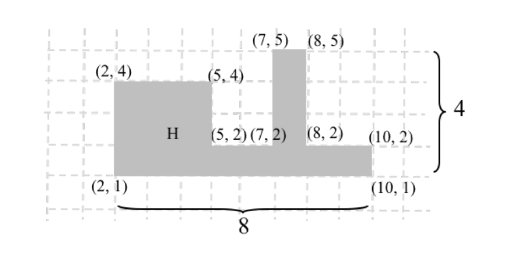
\includegraphics[width=\textwidth]{ProblemA}
Figure 1: a rectangular hole $H$.
\end{center}

In this problem, you are asked to find the area of the smallest rectangular cover that can completely cover $H$. For example, in Figure 1, the output is $32$.

\begin{flushleft}
{\color{red} \textbf{Input}}
\end{flushleft}
The first line is an integer $t$, $1 \leq t \leq 10$, indicating the number of test cases. Each test case starts with one line containing the number $n$. $4 \leq n \leq 100$. of vertices of the hole $H$. Then, $n$ lines follow, each of which contains two integers $x$ and $y$, $0 \leq x, y \leq 1000$, which are the coordinates of the vertices of the hole's polygon in the order they would be visited in a trip around the polygon.

\begin{flushleft}
{\color{red} \textbf{Output}}
\end{flushleft}
For each test case. output the area of the smallest rectangular cover that can completely cover $H$ in one line.

\begin{flushleft}
{\color{red} \textbf{Technical Specification}}
\end{flushleft}
\begin{enumerate}
\item The number of the vertices of $H$, denoted by $n$, is a positive integer between $4$ and $100$.
\item The x-coordinates and y-coordinates of vertices are integers between $0$ and $1000$.
\end{enumerate}

\begin{flushleft}
{\color{red} \textbf{Sample Input}}
\end{flushleft}
\begin{flushleft}
2\\
10\\
10 1\\
10 2\\
8 2\\
8 5\\
7 5\\
7 2\\
5 2\\
5 4\\
2 4\\
2 1\\
4\\
2 1\\
5 1\\
5 4\\
2 4\\
\end{flushleft}

\begin{flushleft}
{\color{red} \textbf{Sample Output}}
\end{flushleft}
\begin{flushleft}
32\\
9\\
\end{flushleft}

\newpage